\chapter[2021 October]{October 2021}

\section[2021/10/04]{Tuesday, 04 October 2021}

\subsection{PCB Assembly}

The PCB for the main robotic controller board as well as the supporting pressure sensor and \ac{LED} breakout boards were received from the JLC PCB board house. The top-view of the main controller board is shown in \FigRef{fig:empty-pcb} below.

\begin{figure}[H]
	\centering
	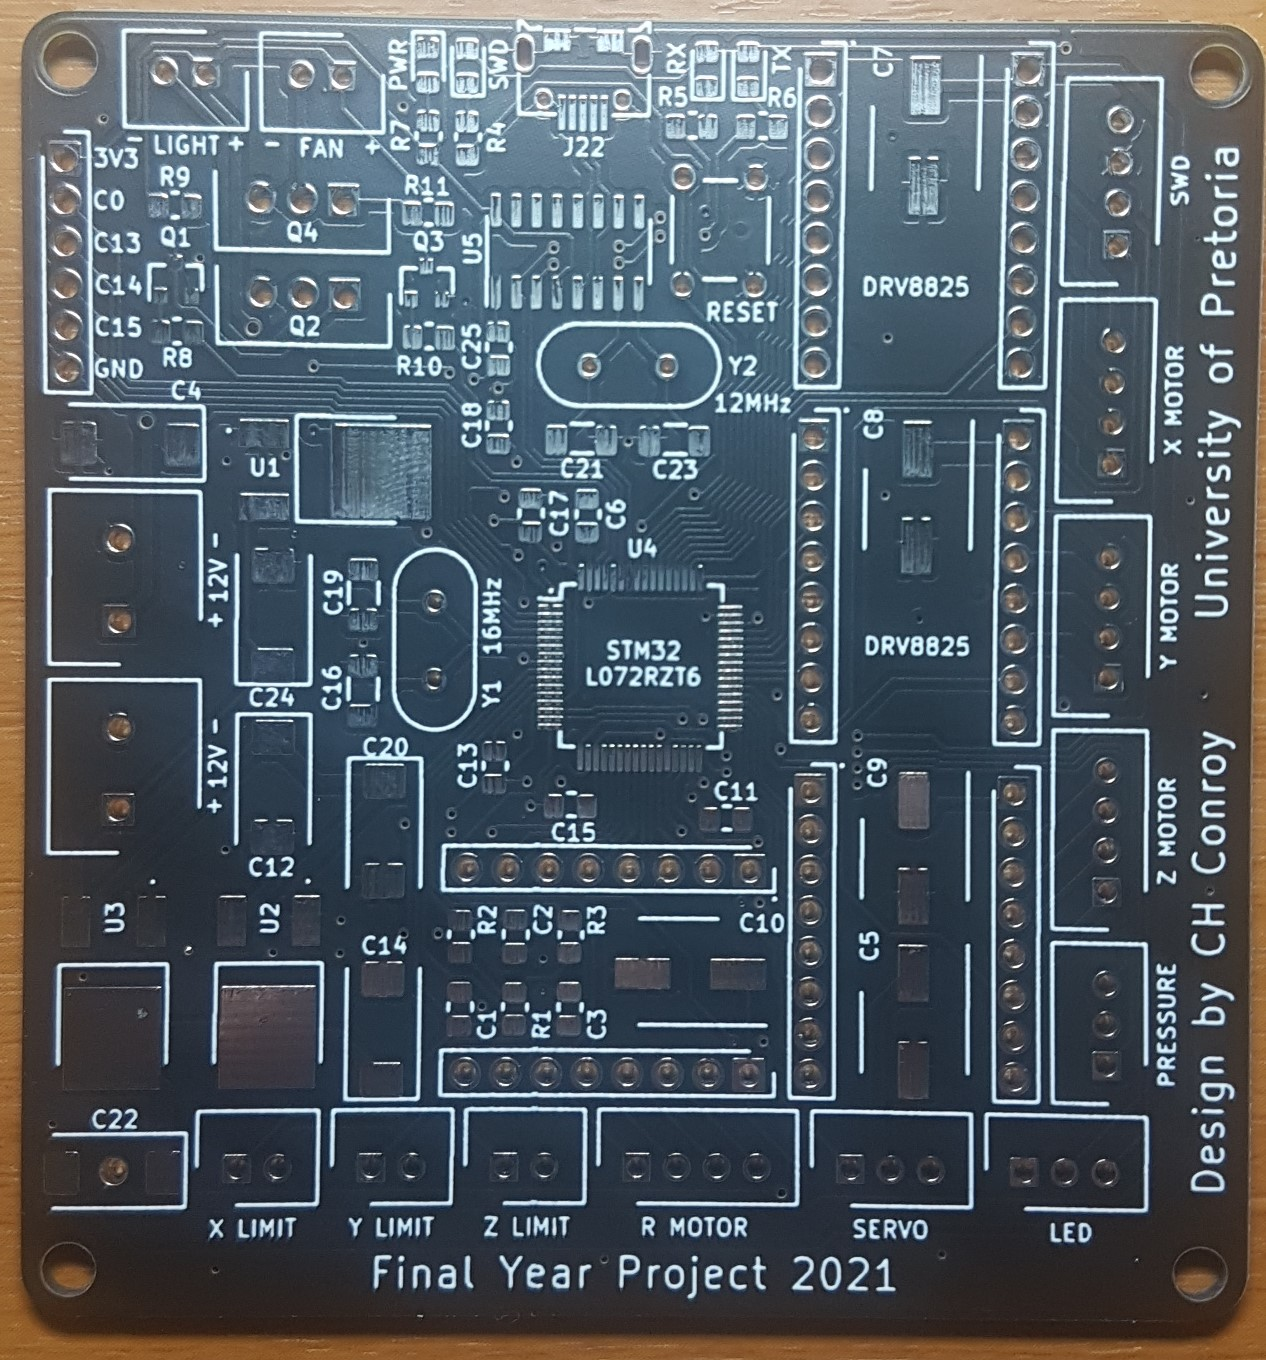
\includegraphics[width=0.6\linewidth]{figures/202110/pcb-board.jpg}
	\caption{Empty PCB board as received from the JLC PCB board house.}
	\label{fig:empty-pcb}
\end{figure}

The components required to assemble the board were acquired prior to the delivery of the PCB board. Due to the close proximity of the components, the components were required to be strategically soldered in order to prevent any obstructions that prevented subsequent components from being soldered in their intended location. Due to the fine pitch (0.5mm) nature of the STM32L072RZT6 microcontroller package, a drag soldering technique was used in conjunction with a significant amount of solder flux to successfully solder the component. The board was cleaned using \ac{IPA} alcohol throughout the soldering process. The assembled PCB board is shown in \FigRef{fig:assembled-pcb} below.

\begin{figure}[H]
	\centering
	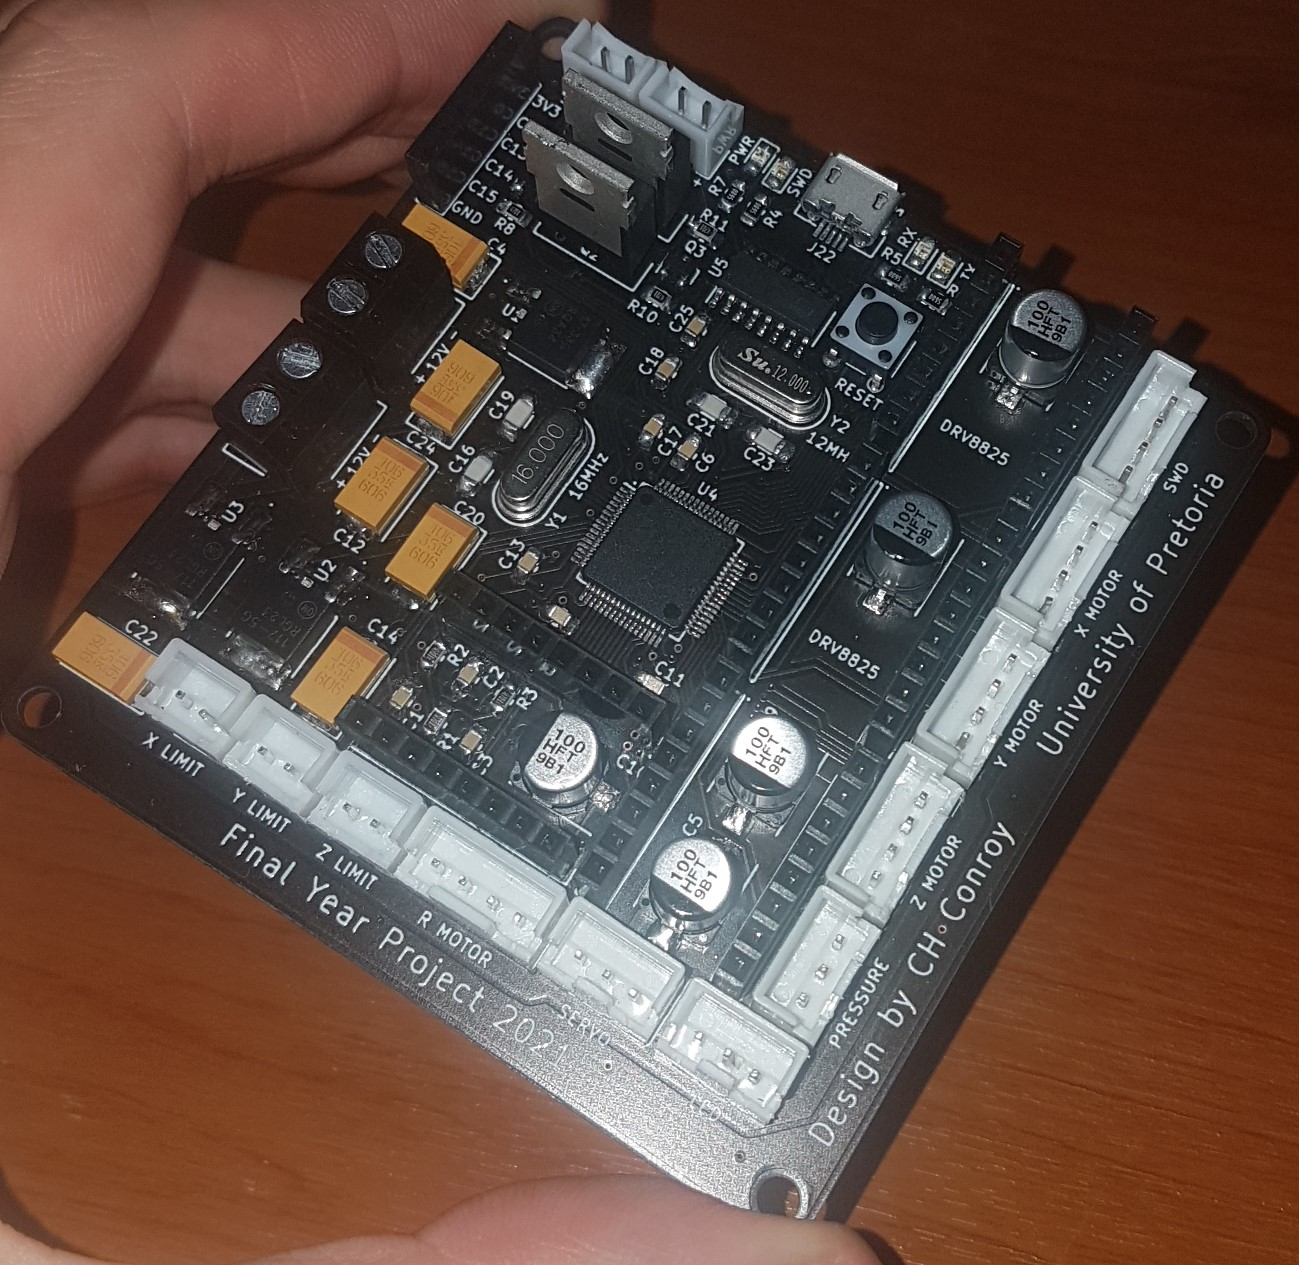
\includegraphics[width=0.6\linewidth]{figures/202110/final-pcb.jpg}
	\caption{PCB board containing all the required components after soldering.}
	\label{fig:assembled-pcb}
\end{figure}

\pendsign

\section[2021/10/10]{Sunday, 10 October 2021}

\subsection{OpenGL}

One of the specifications for this project requires the development of a PC-based \ac{GUI} software component that allows the user to define 3D shapes to be constructed by the robot. Furthermore, the project proposal indicates that this software component must make use of graphical primitives to generate a 3D render of the shape as part of this process. To this extent, the OpenGL specification was selected as the basis for the 3D rendering component. It is noted that OpenGL is only a specification for a graphics \ac{API} and not an implementation in itself. This \ac{API} is usually implemented by the graphics card manufacturers. Furthermore it is noted that can be considered to be a state machine which is described as the graphical context. The behaviour of various OpenGL instructions depends on the state of the OpenGL context.

In order to make use of and learn OpenGL, some supporting software components were required. Firstly, \ac{GLFW} was used to provide a basic window to render OpenGL content in as well as to provide basic mechanisms of interaction with this window through computer peripherals. Secondly, as OpenGL is just a specification, there are a number of versions of drivers that implement this specification. However, the location of these drivers is usually unknown at the point of compilation ad as a result their locations need to be fetched upon execution of the OpenGL dependent program. In order to overcome this issue, \ac{GLAD} was used since it fetches the location of such drivers and makes them available for use in the OpenGL dependent program.

The foundation of rendering using OpenGL rests on the use of vertices. Specifically, a number of vertices are defined as the starting point for various objects to be rendered in 3D. These vertices are assembled into shapes such as triangles depending on the OpenGL context. Triangles were used as the primitive shape created from vertices in this project. Surfaces can be created by generating a number of these shapes adjacent to each other with varying sizes and orientations. These vertices and shapes encounter a number of processes and transformations when being converted from a description in 3D space to a collection of pixels on a 2D computer screen. There are approximately six such steps in this process which are known as the six stages of the graphics pipeline which is shown in \FigRef{fig:graphics-pipeline} below.

\begin{figure}[H]
	\centering
	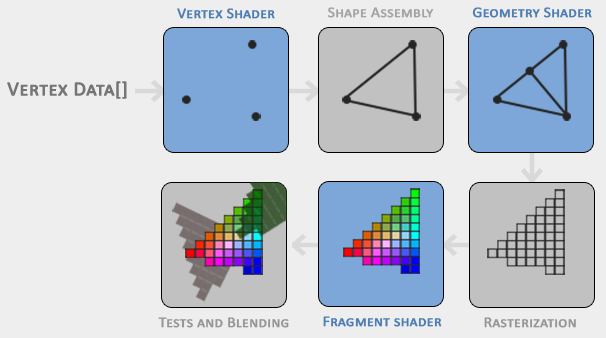
\includegraphics[width=0.7\linewidth]{figures/202110/graphics-pipeline.PNG}
	\caption{Six stages of the graphics pipeline.}
	\label{fig:graphics-pipeline}
\end{figure}

Two of the stages shown in \FigRef{fig:graphics-pipeline} require an implementation to be defined when using OpenGL, namely the vertex shader and the fragment shader. These shaders are written using \ac{GLSL} which is a language similar to C that is used to write shader programs that execute on the graphics card. In order to define the positions and orientations of the various objects to be rendered as well as how they are transformed to 2D space on the screen, a number of coordinate systems and transformation matrices are required. These are shown in \FigRef{fig:graphics-pipeline} below.

\begin{figure}[H]
	\centering
	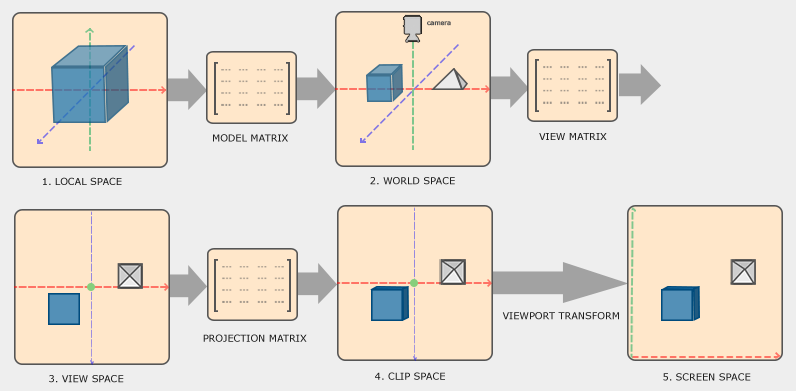
\includegraphics[width=1\linewidth]{figures/202110/transformation-matrices.PNG}
	\caption{Transformation matrices involved in mapping the vertices from local space to screen space.}
	\label{fig:graphics-pipeline}
\end{figure}

The object is described in the local coordinate frame with the origin of the frame of reference usually located somewhere on or within the object. World space is the frame of reference that relates the position, orientation and scale of all the objects to be rendered together. The matrix that maps the local frame to the world frame is known as the model matrix. Similarly, the view of the world, usually thought of as a camera, has its own coordinate system. The world space is mapped to this view space by means of a view matrix. This defines the angle the world is seen from. Lastly, it is noted that the coordinates that are mapped to the screen need to be \ac{NDC} where all vertex values of the coordinate axes are between 0 and 1. Any vertex outside of this space will not be projected onto the screen. As such, this space is called clip space and the projection matrix is used to map from view space to clip space. However, the projection matrix can be used to define the nature of this clip space and as such can be used to control the projection perspective. 

Lastly, the viewport transform is performed to convert the 3D coordinates to 2D coordinates. The former three transforms, namely the model, view and projection matrices, are the transforms that will be manipulated to transform the vertices accordingly. Each of these matrices consist of a translation, rotation and scale sub-component of which the order of operations is important to ensure the correct transform result. By defining cubes using vertex arrays and manipulating these vertices as described above, a pyramid 3D shape that the robot could build was rendered as shown in \FigRef{fig:initial-opengl} below.

\begin{figure}[H]
	\centering
	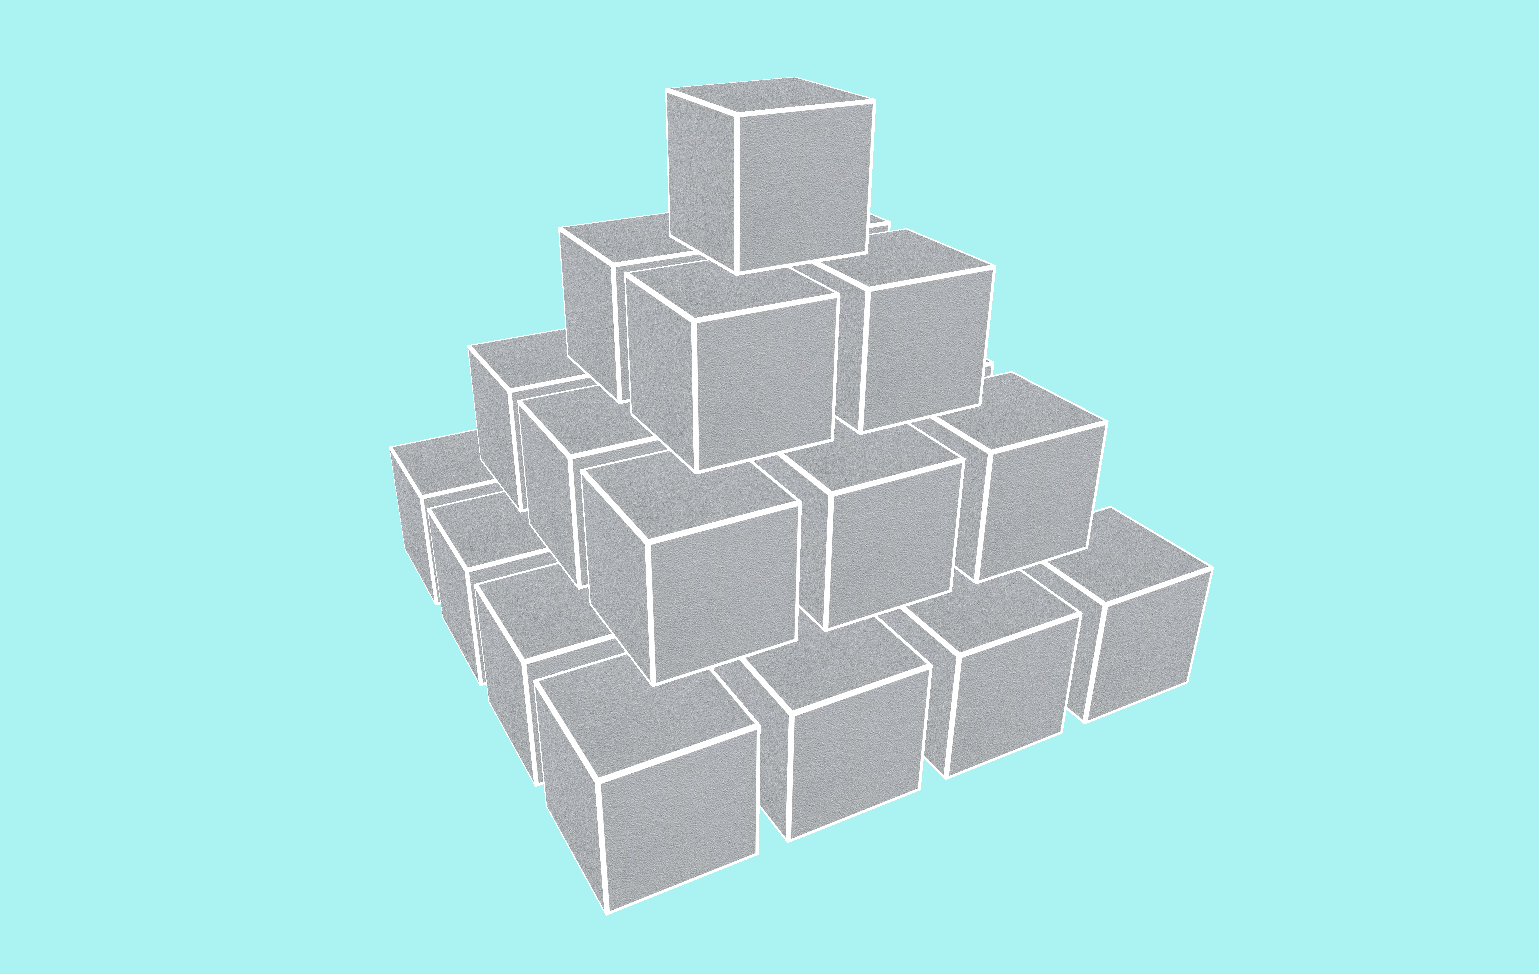
\includegraphics[width=0.8\linewidth]{figures/202110/initial-opengl-shape.PNG}
	\caption{3D render of pyramid shape generated using OpenGL within QT framework.}
	\label{fig:initial-opengl}
\end{figure}

\pendsign

\section[2021/10/14]{Thursday, 14 October 2021}

\subsection{OpenGL Camera}

The next OpenGL component that needed to be implemented after the basic 3D rendering is the camera control. The view matrix is used to map the world space to the camera space. A convenient approach to constructing the view matrix is by using a so-called LookAt matrix $\boldsymbol{V}$. The look at matrix is defined as

\begin{align}
	\boldsymbol{V}=
	\begin{bmatrix}
		R_x & R_y & R_z & 0 \\
		U_x & U_y & U_z & 0 \\
		D_x & D_y & D_z & 0 \\
		0 & 0 & 0 & 1 \\
	\end{bmatrix}
	\begin{bmatrix}
		1 & 0 & 0 & -P_x \\
		0 & 1 & 0 & -P_y \\
		0 & 0 & 1 & -P_z \\
		0 & 0 & 0 & 1 \\
	\end{bmatrix}
\end{align}

where $\boldsymbol{R}$ is the right vector, $\boldsymbol{U}$ is the up vector, $\boldsymbol{D}$ is the direction vector and $\boldsymbol{P}$ is the position vector for the camera in the world space. These vectors defining the $\boldsymbol{V}$ matrix can be obtained from 3 vectors which are much more intuitive to use for camera control. Specifically a position, target (i.e. the point in the world space the camera is pointed towards) and up vector are sufficient to derive a look up matrix. This was used as the basis to form the camera system for this project's implementation. The desired camera behaviour was defined as follows:

\begin{compactitem}
	\item The camera frame x-axis should remain parallel to the world xz plane.
	\item The camera movement about a point should always be on the surface of a dome about that point when not translating or zooming.
	\item As the camera rotates the camera should continue to look at the same focal point.
\end{compactitem}

This behaviour was successfully implemented for the camera.

\subsection{Shape Definition}

The following features were completed regarding the OpenGL 3D shape definition component:

\begin{compactitem}
	\item Camera control by means of computer peripherals was implemented. The right mouse button can be used to control the rotation of the camera about a given focal point. The middle mouse button can be used to translate the camera horizontally in the world scene.
	\item The OpenGL shape render view was integrated with the main software \ac{GUI} component.
	\item The ability for the user to insert and remove shapes from the model as well as the ability for the user to specify the position and rotation of the cube within the 3D model space.
	\item The option to load and save model files.
\end{compactitem}

\pendsign
